\subsection{CU15 Visualizar Refacciones}
En esta ventana, el administrador puede visualizar todas las refacciones que se encuentran dentro del almacén del taller. Esta tabla posee tres columnas, el Número de Inventario de la refacción, la descripción de la misma refacción y por último el vehículo para el que se necesita. En la parte inferior de la ventana tenemos varias opciones:
\begin{itemize}
	\item \textbf{Actualizar Registros:} Una vez que se haya realizado una acción con algún registro de la tabla, el administrador debe de dar click en este botón para que todas las filas y columnas de la tabla se actualicen.
	\item \textbf{Registrar Refacción:} Se despliega una pantalla donde el administrador podrá ingresar los datos necesarios para hacer un registro de una refacción.
	\item \textbf{Modificar Refacción:} En caso de que se necesite modificar por alguna razón un registro de refacción se podrá hacer con esta ocpción.
	\item \textbf{Eliminar Refacción:} Cuando se requiera eliminar un registro de una refacción por la razón que sea, esta opción ayudará al administrador a hacerlo desplegando un mensaje de seguridad.
	\item \textbf{Salir: }El sistema regresará a la ventana del menú del administrador, figura \ref{fig:Pantalla Visualizar Menu Administrador - Vista de Escenarios}. 
\end{itemize}
En caso de que no se seleccione una fila dentro de la tabla y se desee modificar o eliminar algún registro de la refacción se mostrará un mensaje de error y el administrador será enterado del error que está cometiendo. 
\begin{figure}[!h]
	\centering
	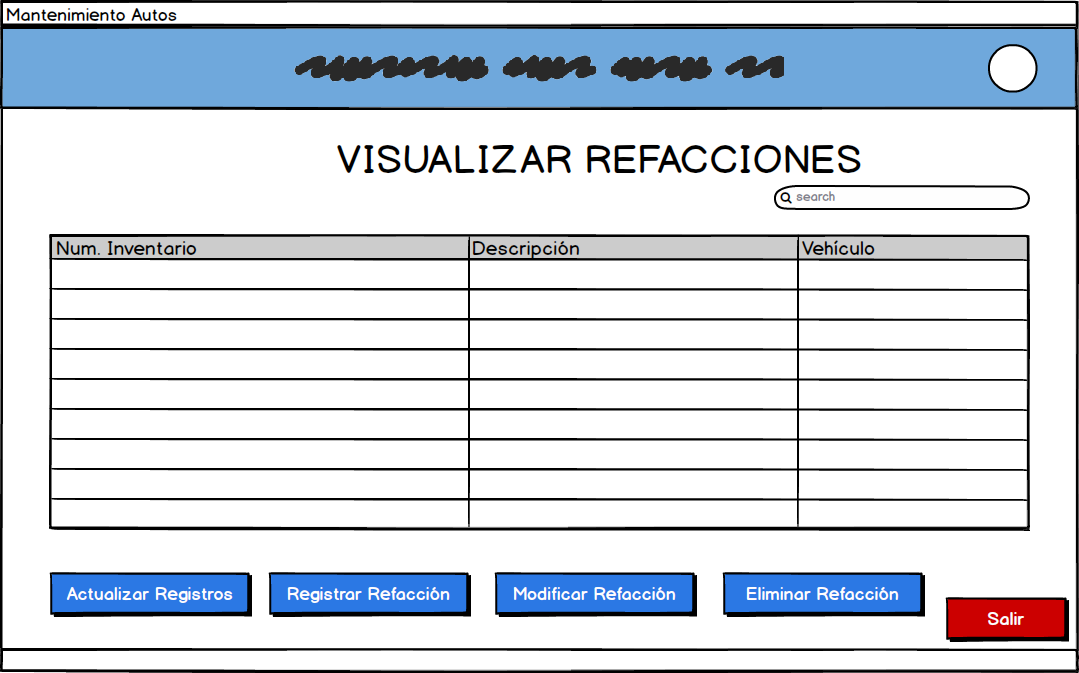
\includegraphics[width=1\textwidth]{./diseno/vescenarios/imagenes/VisualizasRefacciones}
	\caption{Pantalla Visualizar Refacciones Administrador - Vista de Escenarios}
	\label{fig:Pantalla Visualizar Refacciones Administrador - Vista de Escenarios}
\end{figure}
\begin{figure}[!h]
	\centering
	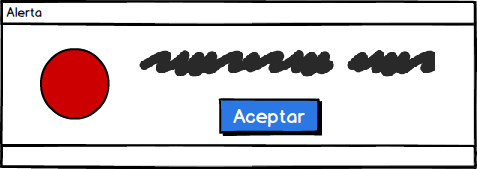
\includegraphics[width=0.5\textwidth]{./diseno/vescenarios/imagenes/alerta}
	\caption{Alerta Refacciones- Vista de Escenarios}
	\label{fig:Alerta Refacciones - Vista de Escenarios}
\end{figure}
\clearpage